\documentclass{../inc/mybibbook}

%%%%%%%%%%%%% Titelseite %%%%%%%%%%%%%%%%%%%%%%%%%%%%%%%%%%%%%%%%%%%%%
%\title{\textcolor{green}{Bibelschule GBSM}}
\author{Schmid Lothar}
\date{2021 -- 2024}
\title{
    \includegraphics[scale=1]{../assets/images/logo.png}\\
    \textbf{Bibel Kommentare}
    \author{Schmid Lothar}
}


%%%%%%%%%%%%%%%%% Beginn Dokument %%%%%%%%%%%%%%%%%%%%%%%%%%%%%%%%%%%%
\setlength{\parindent}{6pt}


\begin{document}
\maketitle
\tableofcontents

\newpage

\section{Allgemein Infos über die Bibel}
\section{Das Alte Testament}
\section{1. Mose Genesis}

\subsection{Kapitel 1}
Das erste Kapitel gibt einen Überblick wie Gott das Universum (Verse: 1 - 5), die Wasser (Verse 6 - 10), die Pflanzen (Verse 11 - 13), die Tage ( Verse 14 - 19), die Tiere (Verse 20 -25) und die Menschen (Verse 26 - 27) geschaffen hat. Die Erschaffung des Menschen ist im 1 Kapitel relativ kurz gehalten. Diese wird dann im Kapitel 2 ausführlicher behandelt.

Jede Schöpfung geschieht an einem Tag. Am Ende des Tages heisst es immer: \textquoteleft{Und es wurde Abend, und es wurde Morgen der fünfte Tag.} 
Das heisst der Tag hatte einen normalen Ablauf. Am Morgen aufstehen mit der Arbeit beginnen und am Abend die Arbeit niederlegen und ab in den Feierabend.

Es wird auch aufgezeigt, dass jeden Abend Gott sein Werk betrachtete und mit seiner Arbeit zu frieden war.

Ich finde das wir aus diesem Kapitel lernen können wie wir unsere Tage gestalten sollten. Am Tag die Arbeit verrichten und nach getaner Arbeit zufrieden auf diese zurückblicken. Es ist auch wichtig, dass wir wirklich in den Feierabend gehen und die Arbeit bis am Morgen wieder ruhen lassen.

Gott hat nicht alles an einem Tag erschaffen um der Rest der Woche frei zu haben. Es ist sehr wichtig, dass wir mit unserem Tag zufrieden sind. Als ehemaliger Bäcker weiss ich, dass die Nachtarbeit sehr anstrengend ist. Da ist es sehr wichtig, dass man sich die Erholung am Tag holt. Dies ist natürlich schwieriger, weil es hell und lauter ist.

\begin{bibeltext}{NEU}{Spr}{4:24}
Entferne Unwarheit aus deinem Mund, die Falschheit von deinen Lippen.
\end{bibeltext}

\subsection{Kapitel 2}
Im zweiten Kapitel wird am Anfang der 7. Tag der Woche beschrieben.
\begin{bibeltext}{Schl}{Gen}{2:3}
	Und Gott segnete den siebten Tag und heiligte ihn, denn an ihm ruhte er von seinem ganzen Werk, das Gott schuf, als er es machte.
\end{bibeltext}
Hier steht ja nirgends, dass der siebte Tag ein Sonntag oder ein Sabbat war. Es heisst einfach, dass Gott nach 6 Tagen arbeiten, diese hingelegt hat. Am siebten Tag hat er geruht. Er ging nicht auf den neuen Meer Surfen, sondern er hat geruht. Welcher Tag das in der Woche ist finde ich unwichtig. Aber es sollte ein Tag in der Woche geruht werden.

An diesem Tag können wir einen Rückblick der Woche machen und Gott für seine Fürsorge danken. In unserem Arbeitssystem ist sicher gestellt, dass wir einen Tag frei haben. Öfters wird dieser Tag aber für einen andere Arbeit benutzt. Es gibt sicher Menschen denen das Geld von sechs Tage Arbeit, zum leben nicht reicht. Es geht aber nicht nur um die Existenz. Bei uns im Wallis war Sonntagsarbeit immer verpönt. Die Nachbarn haben darauf geachtet, dass man nicht Arbeit und zum Gottesdienst geht. Die jungen Bauern von heute kennen das nicht mehr. Die Woche auf der regulären Arbeit, am Wochenende dann auf der Wiese. Aber viele Hobbys arten zu Arbeit aus. Vor allem Sport Wettkampf. Das Training die Leistung alles braucht Substanz und man kommt nicht zur der Ruhe die man braucht um sich zu erholen.

In den restlichen Versen wird dann die Erschaffung des Menschen detaillierter aufgezeigt. Von 4--6 wird nochmals kurz die Schöpfung zusammengefasst und dann die Erschaffung den Menschen aus \textquoteleft{Staub von der Erde}.

Innerhalb seiner Schöpfung pflanzte Gott einen Garten und setzte den Menschen da hinein. In diesem Garten standen auch die zwei verhängnisvollen Bäume \textquoteleft{Baum des Lebens} und \textquoteleft{Baum der Erkenntnis des Guten und Bösen}. Dieser Garten wird der Garten Eden genannt. In diesem Garten lebte der Mensch mit Gott zusammen. Gott hat die Angewohnheit am Abend in Eden spazieren zu gehen. Gott gab aber dem Menschen die Anweisung, dass er die Früchte von dem \textquoteleft{Baum der Erkenntnis des Guten und Bösen}, nicht essen darf.
\begin{bibeltext}{Schl}{Gen}{2:17}
	aber von dem Baum der Erkenntnis des Guten und des Bösen sollst du nicht essen; denn an dem Tag, da du davon isst, musst du gewisslich sterben!\footnote{Die ersten Menschen kannten den Tod noch nicht; er kam erst als Folge der Sünde über den Menschen. \bibleverse{Rom} {5:12}; \bibleverse{Rom} {6:23}; \bibleverse{Eph} {2:1-3}}
\end{bibeltext}

Ab Vers 18 kommen wir zur Erschaffung der Frau. Nachdem der erste Mensch allen Tieren einen Namen gegeben hat und herausgefunden hatte, dass unter den Tieren kein wirklich gegenüber zu finden war, hat Gott aus der Rippe des ersten Menschen die Frau erschaffen.
\begin{bibeltext}{Schl}{Gen}{2:24}
	Darum wird ein Mann seinen Vater und seine Mutter verlassen und seiner Frau anhängen.
\end{bibeltext}
Ein interessanter Satz. Das zeigt mir, dass diese ersten beiden Menschen auch im Garten Eden Kinder bekommen hätten und diese dann später geheiratet hätten. Oder der Autor hat diesen Satz hinzugefügt, um die heutige Hochzeit zwischen Mann und Frau zu erklären. In jeder Kultur werden die Paare verheiratet. Irgend wie hat das Heiraten was. Wieso wollen gleichgeschlechtliche Paare eigentlich immer heiraten? Wieso reicht es ihnen nicht einfach zusammen zu leben? Gesetzlich könnte man das ja einfach regeln. Es muss etwas im Menschen sein das diesem das Bedürfnis gibt, dass eine höhere Instanz die Zustimmung zu dem zusammenleben gibt.

\subsection{Kapitel 3}
In diesem Kapitel wird der Sündenfall des Menschen beschrieben. Die Geschehnisse in diesem Kapitel sind der Grund wieso die Bibel Überhaupt geschrieben werden musste. Nach dem Sündenfall des Menschen, musste Gott den ganzen Heilsplan in Bewegung setzten, um die Menschen wieder in seine Nähe zu ziehen.

Es ist erstaunlich, dass schon diese zwei Menschen schon daran interessiert waren, Macht zu besitzen. Eigentlich ging es doch ihnen gut im Paradies. Hatten alles, aber trotzdem wollten sie mehr. Sie wollten so sein wie Gott. Die Schlange hat es ihnen versprochen. Sie müssen nur von diesem Baum essen.
\begin{bibeltext}{Sch2}{Gen}{3:1}
	Aber die Schlange war listiger als alle Tiere des Feldes, die Gott der Herr gemacht hatte; und sie sprach zur Frau: Sollte Gott wirklich gesagt haben, dass ihr von \textbf{keinem} Baum im Garten essen dürft?
\end{bibeltext}
Das hat doch die Schlange geschickt eingefädelt oder? Sie macht der Frau den Mund richtig wässrig. Kann doch nicht so schlimm sein. Gott will euch doch etwas vorenthalten. \textquoteleft{Ihr werdet sein wie Gott... }. Wollen wir das nicht auch heute noch? Sein wie Gott? Flüstert der Satan uns nicht immer noch ins Ohr, \textquoteleft{Hat er euch wirklich diese strengen Gebote gegeben? Hat Gott verboten Spass zu haben? Er ist doch ein Spielverderber. Hört nicht auf ihn. Ihr seid viel schlauer als er. Mit der Wissenschaft seid ihr die Götter}.
Nachdem beide von dem tollen Baum gegessen haben geschieht es. \textquoteleft{\textbf{Da erkannten sie dass sie nackt waren...}}. Ende letztes Kapitel heisst es: \textquoteleft{und sie waren nackt und schämten sich nicht}. Das ist die Erkenntnis von Gut und Böse. Jetzt sieht der Mensch das Böse vom anderen. Sie schämten sich vor einander, sie konnten sich gegenseitig nicht mehr in die Augen blicken.\\
Als dann Gott sie suchte versteckten sie sich im Garten. Das Raus reden ist typisch für uns Menschen. Der Mann schiebt die Verantwortung auf die Frau und auf Gott. \textquoteleft{Du hast mir die Frau gegeben}. Die schiebt die Schuld auf die Schlange. Also genau so wie wir uns noch Heute aus der Verantwortung winden wollen.

Diese Aktion hatte weitreichende Auswirkungen die wir noch heute spüren. Es kam der Tod, der Schmerz in die Welt. Die Auswirkungen waren so schlimm, dass Gottes Plan schon zu dieser Zeit festgelegt war, seinen Sohn für die Erlösung von uns Menschen zu schicken. Die Menschheit musste aber zuerst vorbereitet werden. Hier tauchen die ersten Hinweise auf das Opfer von seinem Sohn. So sagt Gott zu der Schlange:
\begin{bibeltext}{Sch2}{Gen}{3:15}
	Und ich will Feindschaft setzten zwischen dir und der Frau, zwischen deinem Samen und ihrem Samen: Er wird dir den Kopf zertreten, und du wirst ihn in die Ferse stechen.
\end{bibeltext}
Hier wird gezeigt wie Jesus den Satan besiegt, \textquoteleft{er wird ihm den Kopf zertreten, und du wirst ihm in die Ferse stechen} meint die Kreuzigung Jesus. Im weiteren Verlauf der Bibel werden die Hinweise auf Jesus immer konkreter.
Auch die beiden Menschen bekamen ihre Strafe, mit der wir noch jetzt leben und zu kämpfen haben. Geburtsschmerzen, Krankheit auch die strenge Arbeit zum überleben, hat von an ihren Anfang.

Adam\footnote{Hebr. Adama: Erdboden. Dient als Eigennamen für den Mensch} nannte seine Frau Eva\footnote{Hebr. Chawa: Leben} und Gott stattete die beiden mit Kleider aus Fellen aus. Die Auslegung sagt, dass die Felle das erste Blutopfer für die begangene Sünde des Menschen war. Dar letzte Blutopfer hat Jesus der Christus für uns am Kreuz in Golgotha vollbracht.
\subsection{Kapitel 4}
Eva wurde schwanger und gebar den Kain\footnote{bed. Erwerb}. Später gebar sie einen zweiten Sohn mit dem Namen Abel. Ich glaube das ist das berühmteste Pärchen auf dieser Welt. Kain und Abel. Es heisst hier, Kain war Ackerbauer und Abel ein Schafhirte. Beide brachten dem Herrn ein Opfer dar. Kain von den Früchten der Erde und Abel schlachtete ein Schaf. Gott sah das Opfer von Abel an aber das von Kain nicht. War es wirklich nur darum, dass Kain kein Tier geschlachtet hat? Ich kann das nichst so recht glauben. Kann es nicht auch sein, dass Kain schon immer ein Problemkind war? Als Gott sein Opfer nicht anerkannte, wurde er ja ziemlich zornig auf seinen Bruder. Wenn ich ohne Gott unterwegs bin und gegen ihn sündige, wird es wohl nicht reichen wenn ich ihm einfach ein Opfer darbringe und denke, jetzt ist er wieder zufrieden mit mir. Als er dann sah dass es doch nicht so einfach ist Gott zu beeinflussen, wurde er dann halt sauer. Gott ihn ja darauf aufmerksam gemacht. Er hätte es vor Gott wieder gutmachen können.
\begin{bibeltext}{ELB}{Gen}{4:6-7}
	Und der \herr{} sprach zu Kain: "Warum bist du ergrimmt, und warum und warum hat sich dein Angesicht gesent? Ist es nicht so, dass es sich erhebt, wenn du recht tust?"
\end{bibeltext}
Das ist doch etwas was uns auch immer wieder passiert. Wenn wir merken, dass wir etwas schlimmes getan haben, ducken wir uns und wir dürfen nicht mehr direkt in die Augen schauen? Da gibt es dann Zwei Möglichkeiten, wir biegen das geleistete wieder gerade und bringen es vor Gott oder wir kehren es unter den Tisch und warten bis sich alles als Hass in uns aufgestaut hat. Man wird bitter und wird böse gegenüber der Umwelt. Wer jetzt eher Gewalttätig ist lässt es an anderen raus oder er tut sich selber Gewalt an. Kain ging dann in die grosse weite Welt und gründete dort eine Stadt. Die Nachkommen Kain gründeten die Zivilisation. Adam bekam noch einen weiteren Sohn. Diese Sohn nannte er Set. Aus der Linie Set entstammte Noah.

\subsection{Kapitel 5}
\begin{figure}[ht]
    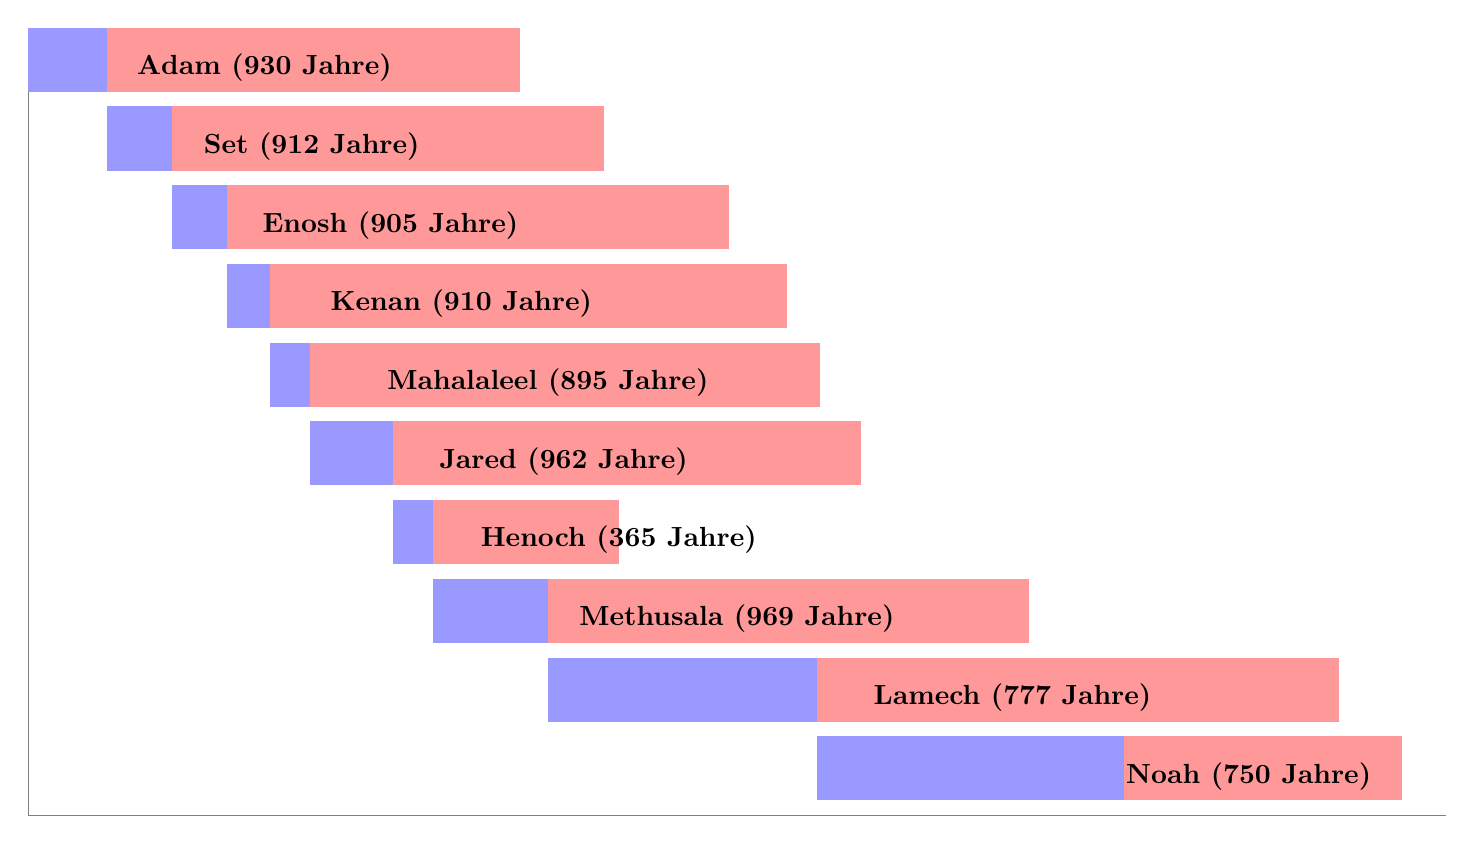
\begin{tikzpicture}
        \draw[gray] (0,0) -- (0mm, 100mm);
        %Adam 130-800 (10.1 - 62.4)
        \filldraw[blue!40] (0,100mm) rectangle(10.1mm,92mm);
        \filldraw[red!40] (10.1mm,100mm) rectangle(62.4mm,92mm) node at (30mm, 92mm) [right, above, black]{\textbf{Adam (930 Jahre)}};
        %Set 105-807 (8.19 - 62.9)
        \filldraw[blue!40] (10.1mm,90mm) rectangle(18.29mm,82mm);
        \filldraw[red!40] (18.29mm,90mm) rectangle(73.0mm,82mm) node at (36mm, 82mm) [right, above, black]{\textbf{Set (912 Jahre)}};
        %Enosch 90 - 815 (7.02 - 63.6)	
        \filldraw[blue!40] (18.29mm,80mm) rectangle (25.31mm,72mm);
        \filldraw[red!40] (25.31mm,80mm) rectangle(88.91mm,72mm) node at (46mm, 72mm) [right, above, black]{\textbf{Enosh (905 Jahre)}};
        %Kenan 70 - 840 (5.46 - 65.52)		
        \filldraw[blue!40] (25.31mm,70mm) rectangle(30.77mm,62mm);
        \filldraw[red!40] (30.77mm,70mm) rectangle(96.29mm,62mm) node at (55mm, 62mm) [right, above, black]{\textbf{Kenan (910 Jahre)}};
        %Mahalaleel 65 - 830 (5.07 - 64.7)
        \filldraw[blue!40] (30.77mm,60mm) rectangle(35.84mm,52mm);
        \filldraw[red!40] (35.84mm,60mm) rectangle(100.54mm,52mm) node at (66mm, 52mm) [right, above, black]{\textbf{Mahalaleel (895 Jahre)}};
        %Jared 162 - 800 (12.6 - 62.4)
        \filldraw[blue!40] (35.84mm,50mm) rectangle(46.44mm,42mm);
        \filldraw[red!40] (46.44mm,50mm) rectangle(105.68mm,42mm) node at (68mm, 42mm) [right, above, black]{\textbf{Jared (962 Jahre)}};
        %Henoch 65 - 300 (5.07 - 23.4)
        \filldraw[blue!40] (46.44mm,40mm) rectangle(51.51mm,32mm);
        \filldraw[red!40] (51.51mm,40mm) rectangle(74.91mm,32mm) node at (75mm, 32mm) [right, above, black]{\textbf{Henoch (365 Jahre)}};
        %Methusalah 187 - 782 (14.58 - 60.99)
        \filldraw[blue!40] (51.51mm,30mm) rectangle(66.09mm,22mm);
        \filldraw[red!40] (66.09mm,30mm) rectangle(127.08mm,22mm) node at (90mm, 22mm) [right, above, black]{\textbf{Methusala (969 Jahre)}};
        %Lamech 182 - 595 (14.19 - 46.41)
        \filldraw[blue!40] (66.09mm,20mm) rectangle(100.28mm,12mm);
        \filldraw[red!40] (100.28mm,20mm) rectangle(166.37mm,12mm) node at (125mm, 12mm) [right, above, black]{\textbf{Lamech (777 Jahre)}};
        % Noah 500 - 450 (39 - 35.1)
        \filldraw[blue!40] (100.28mm,10mm) rectangle(139.28mm,2mm);
        \filldraw[red!40] (139.28mm,10mm) rectangle(174.38mm,2mm) node at (155mm, 2mm) [right, above, black]{\textbf{Noah (750 Jahre)}};

        \draw[gray] (0,0) -- (180mm, 0mm);
    \end{tikzpicture}
    \caption{Lebensjahre bis Noah}
    \label{balken_alter}
\end{figure}
In diesem Kapitel wird das Geschlechtsregister Adams bis Noah aufgelistet. Die Menschen wurden zu der Zeit ziemlich alt. Durch dieses Alter gab es eine Spezielle konstellation.
Es ist interessant zu sehen (Abbildung: \ref{balken_alter}), wie Noah noch die Geburt von Lamech knapp miterleben konnte. Ich glaube zwar nicht, dass die sich nach so langer Zeit noch gekannt haben, aber es ist spannend. Am Ende das blauen Balken wurde dann der erste Sohn geboren, oder wenigsten die Person die die direkte Linie zu Jesus weiter führte.
Dieses Kapitel endet mit der Erwähnung von Noah und es werden seine Söhne Sem, Ham, Japhet aufgelistet.
\subsection{Kapitel 6}
Am Anfang des Kapitels wird erklärt, warum Gott die Menschen vernichten wollte. Es steht nirgends, dass er die Erde vernichten will, sondern nur die Lebewesen auf dieser Erde. Gott fand, das alle Menschen schlecht sind. In Vers 6 steht folgendes.
\begin{bibeltext}{ELB}{Gen}{6:6}
    Und es reute den \herr , dass er den Menschen gemacht hatte auf der Erde, und es schmerzte ihn in sein Herz hinein.
\end{bibeltext}
In Vers 7 steht, dass er nicht nur die Menschen vernichten will sondern auch alle Tier auf dieser Erde. Und dann in Vers 8.
\begin{bibeltext}{ELB}{Gen}{6:7}
    Noah aber fand Gnade in den Augen des Herrn.
\end{bibeltext}
Auf der ganzen Erde nur ein Mann. Dieser eine Mann wird als gerechter und vollkommener Mann unter seinen Zeitgenossen dargestellt. Durch diesen gerechten Menschen wurden dann auch die Tier nach ihrer Art gerettet. Für die Rettung der Menschen und der Tiere gab ihm Gott den Auftrag ein Schiff zu bauen. Mit dem Schiff und dem Regen fängt eine Geschichte an, die mit der Wiederkunft Jesus im neuen Testament vergleichbar ist. Nur mit einer Sintflut und einem grossen Schiff, kann so eine parallele zu unserer heutigen Zeit unsere Erlösung mit Jesus Christus bildlich dargestellt werden.
\begin{figure}[ht]
    \begin{tabular}{lcl}
        Schiff & = & Jesus            \\
        Wasser & = & ungläuber Mensch \\
        Noah   & = & gläubige Mensch  \\
    \end{tabular}
\end{figure}
Noah hat Gott gehorcht und das Schiff gebaut. Die restliche Menschheit wollte sich nicht von einem Gott etwas sagen lassen. Da sind wir schlauer. Uns geht es ja gut, für was brauchen wir noch einen Gott? Sollen wir und die Mühe machen und ein Schiff zusammen zimmern? Läuft doch alles so prima. Eines Tages fing es an zu regnen. Naja ein bisschen Regen wieso sich Sorgen machen. Der Regen wurde aber immer schlimmer.

Das passiert doch auch heute. Mehr Überschwemmungn, mehr Krankheiten, mehr Unruhen und Unzufriedenheit in der Menschheit. Perspektivlosigkeit, werden mit Versuchen den Weltraum zu ergründen überbrückt. Von Menschen gemachter Klimawandel? Vielleicht ist es auch ein von Gott gemachter Klimawandel und es geht wie in der Offenbarung beschrieben langsam dem Ende entgegen? Macht man sich die Mühe mit Jesus Christus unterwegs zu sein, wird man ausgelacht. \textbf{Wir} haben alles im Griff. \textbf{Wir} brauchen niemand, ein bisschen CO\textsuperscript{2} weniger in die Luft jagen und schon wird es uns wieder besser gehen. Kann sein, dass es so wird, muss aber nicht. Es kann aber auch wie zu Noahs Zeiten werden, dass wir besser auf Jesus vertrauen sollten und so in die Arche gelangen um gerettet zu werden.
\subsection{Kapitel 7}
In diesem Kapitel geht es in die Arche. Jetzt fordert Gott Noah auf das Schiff zu füllen und selber in die Arche zu steigen. Gott schickt ein Pärchen von jeder Tierart.

Mit Noah und den Tieren, steigen auch seine Frau, seine 3 Söhne Sem, Ham und Japhet mit ihren Frauen in die Arche ein. Interessant ist, dass Gott im Vers 2 schon hier von reinen und unreinen Tieren spricht. Von den reinen soll er je 7 von jeder Tierart und von den Männchen und Weibchen mitnehmen. Von den unreinen je ein Pärchen. Welche Tiere rein und unrein waren wird nicht verraten. Von den reinen Tieren wurde dann in 
\textquoteleft{{Gen}{8:20} ein Opfer für den \herr n dargebracht.}
    

Noah war 600 Jahre und zwei Monate alt als das Unwetter begann. Es wird nicht nur Regen beschrieben, sondern das Wasser kam von unten und von Oben. Es taten sich alle Brunnen in der grossen Tiefe auf. Der Regen kam dann noch zusätzlich. Es waren riesige Massen an Wasser in kurzer Zeit, welche die Erde überschwemmte. Alle Menschen und Tiere auf dem Land kamen ums leben. Allein Noah und die Passagiere auf der Arche überlebten dieses Inferno.

So wird es auch in den letzten Tagen sein. Viele werde in den letzten Tagen draussen stehen und verloren gehen. Sie werden überrascht sein. Sie werden wütend sein. Trotzdem werden sie nicht an Gott glauben. Sie werden das Unwetter allem anderen zuschieben nur nicht Gott und an seine Rettung glauben. Aus Frust werden sie die verfolgen die an Jesus Christus als den Erlöser glauben. Sie werden sehen, dass diese etwas an sich haben, was sie beruhigt. Wie viele sind der Arche nach geschwommen? Wie viele wollten nachträglich noch auf das Schiff klettern? Viele wurden überrascht. Viele wussten nichts von dem Schiff oder haben das wohl als Geschichte oder Märchen abgetan. Als der Regen anfing haben sie das wohl einem Klimawandel zugeschrieben. Ist unser Klimawandel auch Zeichen Gottes? Bestimmt, es fällt uns ja kein Haar vom Kopf ohne dass er davon weiss.

Das Wasser blieb 150 Tage hoch über der Erde. Es heisst, das Wasser stieg 15 Ellen über den höchsten Berg der Erde. Da war kein entkommen für die Landlebewesen. Alles auf der Erde wurde getötet. Das interessante ist, dass alle Kulturen auf dieser Erde ein Sintflut kennen.

Das Sterben im Wasser war sicher nicht angenehm, aber da alle Menschen auf der Erde gestorben sind gab es auch kein Leid. Das Leid entsteht bei den Zurückgebliebenen, bei diesen ist der Schmerz des alleine seins und verlassen sein gross. Wenn alle Tod sind passiert das nicht. Es ist die Hoffnung der Christen sich eines Tages wieder zu sehen. Dies mildert der Schmerz. Und dass die Person die gestorben ist, es jetzt besser hat als im Leben. Wenn man daran glaubt, dass einen die Würmer fressen kann schon verzweifeln.
\subsection{Kapitel 8}
Zu Beginn des Regens war Noah 600 Jahre alt. Noah war 371 Tage auf diesem Schiff, bis der \herr ihm befohlen das Schiff wieder zu verlassen. Es war eine lange Zeit auf dem Schiff und sicher nicht angenehm. Die psychische Belastung, der Gestank und es war sicher auch laut mit diesen ganzen Tieren. So ist es auch verständlich, dass Noah ungedultig wurde und schon mal einen Raben ausschickte um eine Prüfung der Verhältnisse vor zu nehmen. Als dann der Rabe nicht mehr zurück kam, hat er dann eine Taube im Wochenrhythmus ausgeschickt. Als die dann mit einem Ölblatt zurück kam, konnte er sich vorstellen, dass es wohl nicht mehr so lange geht. Es ging aber noch zwei Monate bis Gott ihn aus der Arche liess.

Es ist doch bei uns auch so. Wir werden sehr Ungeduldig wenn wir in Bedrängnis oder in Not sind. Ist ja auch verständlich. Wer hat schon gerne wenn es ihm schlecht geht? Die folgen für Noah wären fatal gewesen, wäre er zu früh aus dem Schiff gestiegen. Er hätte noch nicht überleben können. Wenn wir Ungeduldig werden und selber vorwärts machen wollen kann das schief gehen. Gott kennt den genauen Zeitpunkt wann er uns wieder auf die Welt los lassen kann ohne das wir schaden davon nehmen. So auch bei Noah. Als Gott ihm sagte, du kannst jetzt raus, war die Welt wieder so hergestellt, dass Noah, seine Familie und die Tiere wieder ohne Gefahr leben konnten. Diese Geduld müssen wir lernen. In unserer schnelllebigen Zeit ist es noch viel schwieriger die Geduld zu waren. Aber um so wichtiger. Es heisst ja nicht, dass wir nicht fragen können, oder informationen sammeln. Der Herr war nicht beleidigt als Moses sein Vögel ausgesandt hat. Er kennt unsere Herzen und weiss genau aus welchem Grund wir irgendwas machen. Aber, wir sollten auf die Freigabe des Herrn warten, bevor wir aus dem Schiff aussteigen. Der Herr gab Noah den Aufrag Fruchtbar zu sein und die Erde zu bevölkern. Auch die Apostel und jetzt wir bekamen diesen Auftrag. Bei Himmelfahrt Jesus sagte er zu den Aposteln. 
\begin{bibeltext}{Elb}{Apg}{1:8}
	Aber ihr werdet Kraft empfangen, wenn der Heilige Geist auf euch gekommen ist; und ihr werdet meine Zeugen sein, sowohl in Jerusalem als auch in ganz Judäa und Samaria und bis an das Ende der Erde.
\end{bibeltext} 
Die Apostel mussten auch eine Durststrecke durchleben nach dem Tod von Jesus. Sie brauchten auch Gedult und Jesus hat sie 40 Tage gelehrt. Danach war der Weg zwar immer noch steinig, aber durch die Hilfe des Heiligen Geistes kamen sie durch alle Berdrängnis.

Was hat Noah als erstes gemacht? Er hat Gott einen Altar gebaut und im Dankopfer dargebracht. Er hat sich nicht auf den Boden gesetzt und mit seinem Schicksal gehadert. Er wusste mit Gott wird das schon gehen. Er hat Gott gedankt, für sein Treue und Gnade ihm und seiner Familie gegenüber. Wie oft danken wir auch wenn es uns nicht so gut geht? Trozdem wir keinen Ausgang mehr sehen?

\section{Das Neue Testament}
%\section{NT Kommentare}
\section{Allgemein Infos über die Bibel}

\printbibliography

\end{document}